\documentclass[aspectratio=169,11pt,xcolor=table]{beamer}

\usetheme{default}
\usecolortheme{default}
\setbeamertemplate{navigation symbols}{}
\setbeamertemplate{footline}[frame number]
\setbeamercolor{title}{fg=black}
\setbeamercolor{frametitle}{fg=black,bg=white}
\setbeamercolor{block title}{fg=black,bg=black!8}
\setbeamercolor{block body}{fg=black,bg=black!3}
\setbeamerfont{frametitle}{series=\bfseries,size=\Large}
\setbeamerfont{title}{series=\bfseries,size=\LARGE}

\usepackage[utf8]{inputenc}
\usepackage[T1]{fontenc}
\usepackage{amsmath,amssymb,bm}
\usepackage{booktabs}
\usepackage{array}
% \usepackage{xcolor} % Removed: Beamer loads this automatically. We passed 'xcolor=table' to \documentclass instead.
\usepackage{tikz}
\usetikzlibrary{shapes.geometric}
\usepackage{pgfplots}
\usepackage{graphicx}
\usepackage{hyperref}
\pgfplotsset{compat=1.18}
\usetikzlibrary{arrows.meta,positioning,calc,fit,matrix}

% -----------------------------------------------------------------------------
% Raster palette: same family/style as the supplied article TeX.
% -----------------------------------------------------------------------------
\definecolor{lowblue}{RGB}{225,240,255}
\definecolor{midblue}{RGB}{120,180,230}
\definecolor{highblue}{RGB}{15,90,160}
\definecolor{lowgreen}{RGB}{230,245,230}
\definecolor{midgreen}{RGB}{120,190,120}
\definecolor{highgreen}{RGB}{20,120,40}
\definecolor{loworange}{RGB}{255,240,220}
\definecolor{midorange}{RGB}{245,170,80}
\definecolor{highorange}{RGB}{190,80,20}
\definecolor{lowred}{RGB}{255,230,230}
\definecolor{midred}{RGB}{240,120,120}
\definecolor{highred}{RGB}{170,20,40}
\definecolor{purpleA}{RGB}{235,225,245}
\definecolor{purpleB}{RGB}{165,120,200}
\definecolor{purpleC}{RGB}{90,40,140}
\definecolor{marginA}{RGB}{245,245,210}
\definecolor{marginB}{RGB}{220,205,95}
\definecolor{marginC}{RGB}{145,120,20}
\definecolor{clusterone}{RGB}{225,240,255}
\definecolor{clustertwo}{RGB}{255,230,190}
\definecolor{clusterthree}{RGB}{230,245,220}
\definecolor{clusterfour}{RGB}{245,220,245}
\definecolor{darkink}{RGB}{25,25,25}
\definecolor{muted}{RGB}{90,90,90}
\definecolor{wqblue}{RGB}{225,240,255}
\definecolor{ecogreen}{RGB}{225,245,225}
\definecolor{memorange}{RGB}{255,236,210}
\definecolor{organismpurple}{RGB}{238,228,248}
\definecolor{marginyellow}{RGB}{255,247,190}
\definecolor{ampred}{RGB}{255,225,225}
\definecolor{regimeblue}{RGB}{230,235,255}
\definecolor{muted}{RGB}{80,80,80}
\definecolor{ViableGreen}{RGB}{46,125,50}
\definecolor{ViableBlue}{RGB}{25,118,210}
\definecolor{PathRed}{RGB}{198,40,40}
\definecolor{PathOrange}{RGB}{239,108,0}
\definecolor{PressurePurple}{RGB}{123,31,162}
\definecolor{SoftGrey}{RGB}{245,245,245}
\definecolor{BarrierGrey}{RGB}{90,90,90}
\definecolor{ecogreen}{RGB}{218,244,222}
\definecolor{debpurple}{RGB}{234,222,246}
\definecolor{waterblue}{RGB}{220,238,255}
\definecolor{burdenorange}{RGB}{255,232,202}
\definecolor{marginyellow}{RGB}{255,246,184}
\definecolor{ampred}{RGB}{255,224,224}
\definecolor{speciesgrey}{RGB}{239,239,239}
\definecolor{darkgrey}{RGB}{70,70,70}


% -------------------------------------------------------------------------
% Mini raster helpers: 3x3 pseudo-rasters
% -------------------------------------------------------------------------
\newcommand{\RasterC}[4]{%
	\begin{scope}[shift={(#1,#2)}]
		\foreach \i/\j/\col in {
			0/0/blue!75, 1/0/teal!70, 2/0/green!55,
			0/1/blue!70, 1/1/teal!65, 2/1/green!50,
			0/2/blue!60, 1/2/teal!55, 2/2/green!45
		}{
			\fill[\col] (\i*0.15,\j*0.15) rectangle ++(0.15,0.15);
		}
		\draw[#4,thick] (0,0) rectangle (0.45,0.45);
		\fill[white] (0.23,0.22) circle (0.035);
		\draw[black] (0.23,0.22) circle (0.035);
		\node[font=\tiny,above] at (0.225,0.48) {#3};
	\end{scope}
}

\newcommand{\RasterB}[4]{%
	\begin{scope}[shift={(#1,#2)}]
		\foreach \i/\j/\col in {
			0/0/purple!80, 1/0/magenta!70, 2/0/orange!70,
			0/1/purple!90, 1/1/red!75,     2/1/yellow!65,
			0/2/purple!80, 1/2/magenta!65, 2/2/orange!55
		}{
			\fill[\col] (\i*0.15,\j*0.15) rectangle ++(0.15,0.15);
		}
		\draw[#4,thick] (0,0) rectangle (0.45,0.45);
		\fill[white] (0.29,0.18) circle (0.035);
		\draw[black] (0.29,0.18) circle (0.035);
		\node[font=\tiny,above] at (0.225,0.48) {#3};
	\end{scope}
}

\newcommand{\RasterAxis}[4]{%
	\begin{scope}[shift={(#1,#2)}]
		\foreach \i/\j/\col in {
			0/0/purple!15, 1/0/purple!35, 2/0/purple!55,
			0/1/purple!25, 1/1/purple!60, 2/1/purple!75,
			0/2/purple!10, 1/2/purple!30, 2/2/purple!45
		}{
			\fill[\col] (\i*0.15,\j*0.15) rectangle ++(0.15,0.15);
		}
		\draw[#4,thick] (0,0) rectangle (0.45,0.45);
		\fill[white] (0.25,0.24) circle (0.03);
		\draw[black] (0.25,0.24) circle (0.03);
		\node[font=\tiny,above] at (0.225,0.48) {#3};
	\end{scope}
}

\newcommand{\RasterMargin}[4]{%
	\begin{scope}[shift={(#1,#2)}]
		\foreach \i/\j/\col in {
			0/0/green!75, 1/0/green!70, 2/0/green!60,
			0/1/teal!65,  1/1/green!60, 2/1/yellow!45,
			0/2/blue!55,  1/2/teal!55,  2/2/green!50
		}{
			\fill[\col] (\i*0.15,\j*0.15) rectangle ++(0.15,0.15);
		}
		\draw[#4,thick] (0,0) rectangle (0.45,0.45);
		\fill[white] (0.26,0.22) circle (0.03);
		\draw[black] (0.26,0.22) circle (0.03);
		\node[font=\tiny,above] at (0.225,0.48) {#3};
	\end{scope}
}

\newcommand{\RasterAmplification}[4]{%
	\begin{scope}[shift={(#1,#2)}]
		\foreach \i/\j/\col in {
			0/0/purple!80, 1/0/red!70,    2/0/orange!65,
			0/1/magenta!75,1/1/orange!75, 2/1/yellow!75,
			0/2/purple!70, 1/2/red!70,    2/2/orange!70
		}{
			\fill[\col] (\i*0.15,\j*0.15) rectangle ++(0.15,0.15);
		}
		\draw[#4,thick] (0,0) rectangle (0.45,0.45);
		\fill[white] (0.29,0.18) circle (0.03);
		\draw[black] (0.29,0.18) circle (0.03);
		\node[font=\tiny,above] at (0.225,0.48) {#3};
	\end{scope}
}


\newcommand{\cellbox}[2]{\fill[#1] #2 rectangle ++(0.8,0.8);}
\newcommand{\gridframe}{\draw[black!40,step=0.8] (0,0) grid (4,4);}
\newcommand{\rastlabel}[1]{\node[font=\scriptsize,align=center] at (2,-0.35) {#1};}
\newcommand{\smalltag}[1]{\node[font=\tiny,align=center,text=black!65] at (2,4.35) {#1};}

\newcommand{\drawRasterCOne}{%
	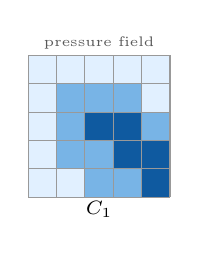
\begin{tikzpicture}[scale=0.45]
		\cellbox{lowblue}{(0,0)} \cellbox{lowblue}{(0.8,0)} \cellbox{midblue}{(1.6,0)} \cellbox{midblue}{(2.4,0)} \cellbox{highblue}{(3.2,0)}
		\cellbox{lowblue}{(0,0.8)} \cellbox{midblue}{(0.8,0.8)} \cellbox{midblue}{(1.6,0.8)} \cellbox{highblue}{(2.4,0.8)} \cellbox{highblue}{(3.2,0.8)}
		\cellbox{lowblue}{(0,1.6)} \cellbox{midblue}{(0.8,1.6)} \cellbox{highblue}{(1.6,1.6)} \cellbox{highblue}{(2.4,1.6)} \cellbox{midblue}{(3.2,1.6)}
		\cellbox{lowblue}{(0,2.4)} \cellbox{midblue}{(0.8,2.4)} \cellbox{midblue}{(1.6,2.4)} \cellbox{midblue}{(2.4,2.4)} \cellbox{lowblue}{(3.2,2.4)}
		\cellbox{lowblue}{(0,3.2)} \cellbox{lowblue}{(0.8,3.2)} \cellbox{lowblue}{(1.6,3.2)} \cellbox{lowblue}{(2.4,3.2)} \cellbox{lowblue}{(3.2,3.2)}
		\gridframe\rastlabel{$C_1$}\smalltag{pressure field}
\end{tikzpicture}}

\newcommand{\drawRasterCTwo}{%
	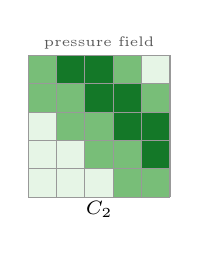
\begin{tikzpicture}[scale=0.45]
		\cellbox{lowgreen}{(0,0)} \cellbox{lowgreen}{(0.8,0)} \cellbox{lowgreen}{(1.6,0)} \cellbox{midgreen}{(2.4,0)} \cellbox{midgreen}{(3.2,0)}
		\cellbox{lowgreen}{(0,0.8)} \cellbox{lowgreen}{(0.8,0.8)} \cellbox{midgreen}{(1.6,0.8)} \cellbox{midgreen}{(2.4,0.8)} \cellbox{highgreen}{(3.2,0.8)}
		\cellbox{lowgreen}{(0,1.6)} \cellbox{midgreen}{(0.8,1.6)} \cellbox{midgreen}{(1.6,1.6)} \cellbox{highgreen}{(2.4,1.6)} \cellbox{highgreen}{(3.2,1.6)}
		\cellbox{midgreen}{(0,2.4)} \cellbox{midgreen}{(0.8,2.4)} \cellbox{highgreen}{(1.6,2.4)} \cellbox{highgreen}{(2.4,2.4)} \cellbox{midgreen}{(3.2,2.4)}
		\cellbox{midgreen}{(0,3.2)} \cellbox{highgreen}{(0.8,3.2)} \cellbox{highgreen}{(1.6,3.2)} \cellbox{midgreen}{(2.4,3.2)} \cellbox{lowgreen}{(3.2,3.2)}
		\gridframe\rastlabel{$C_2$}\smalltag{pressure field}
\end{tikzpicture}}

\newcommand{\drawRasterCThree}{%
	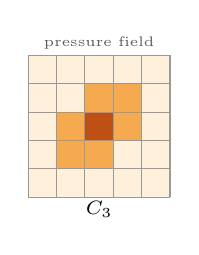
\begin{tikzpicture}[scale=0.45]
		\cellbox{loworange}{(0,0)} \cellbox{loworange}{(0.8,0)} \cellbox{loworange}{(1.6,0)} \cellbox{loworange}{(2.4,0)} \cellbox{loworange}{(3.2,0)}
		\cellbox{loworange}{(0,0.8)} \cellbox{midorange}{(0.8,0.8)} \cellbox{midorange}{(1.6,0.8)} \cellbox{loworange}{(2.4,0.8)} \cellbox{loworange}{(3.2,0.8)}
		\cellbox{loworange}{(0,1.6)} \cellbox{midorange}{(0.8,1.6)} \cellbox{highorange}{(1.6,1.6)} \cellbox{midorange}{(2.4,1.6)} \cellbox{loworange}{(3.2,1.6)}
		\cellbox{loworange}{(0,2.4)} \cellbox{loworange}{(0.8,2.4)} \cellbox{midorange}{(1.6,2.4)} \cellbox{midorange}{(2.4,2.4)} \cellbox{loworange}{(3.2,2.4)}
		\cellbox{loworange}{(0,3.2)} \cellbox{loworange}{(0.8,3.2)} \cellbox{loworange}{(1.6,3.2)} \cellbox{loworange}{(2.4,3.2)} \cellbox{loworange}{(3.2,3.2)}
		\gridframe\rastlabel{$C_3$}\smalltag{pressure field}
\end{tikzpicture}}

\newcommand{\drawRasterAxis}{%
	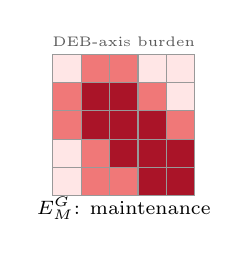
\begin{tikzpicture}[scale=0.45]
		\cellbox{lowred}{(0,0)} \cellbox{midred}{(0.8,0)} \cellbox{midred}{(1.6,0)} \cellbox{highred}{(2.4,0)} \cellbox{highred}{(3.2,0)}
		\cellbox{lowred}{(0,0.8)} \cellbox{midred}{(0.8,0.8)} \cellbox{highred}{(1.6,0.8)} \cellbox{highred}{(2.4,0.8)} \cellbox{highred}{(3.2,0.8)}
		\cellbox{midred}{(0,1.6)} \cellbox{highred}{(0.8,1.6)} \cellbox{highred}{(1.6,1.6)} \cellbox{highred}{(2.4,1.6)} \cellbox{midred}{(3.2,1.6)}
		\cellbox{midred}{(0,2.4)} \cellbox{highred}{(0.8,2.4)} \cellbox{highred}{(1.6,2.4)} \cellbox{midred}{(2.4,2.4)} \cellbox{lowred}{(3.2,2.4)}
		\cellbox{lowred}{(0,3.2)} \cellbox{midred}{(0.8,3.2)} \cellbox{midred}{(1.6,3.2)} \cellbox{lowred}{(2.4,3.2)} \cellbox{lowred}{(3.2,3.2)}
		\gridframe\rastlabel{$E_{M}^{G}$: maintenance}\smalltag{DEB-axis burden}
\end{tikzpicture}}

\newcommand{\drawRasterMargin}{%
	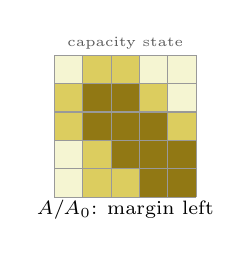
\begin{tikzpicture}[scale=0.45]
		\cellbox{marginA}{(0,0)} \cellbox{marginB}{(0.8,0)} \cellbox{marginB}{(1.6,0)} \cellbox{marginC}{(2.4,0)} \cellbox{marginC}{(3.2,0)}
		\cellbox{marginA}{(0,0.8)} \cellbox{marginB}{(0.8,0.8)} \cellbox{marginC}{(1.6,0.8)} \cellbox{marginC}{(2.4,0.8)} \cellbox{marginC}{(3.2,0.8)}
		\cellbox{marginB}{(0,1.6)} \cellbox{marginC}{(0.8,1.6)} \cellbox{marginC}{(1.6,1.6)} \cellbox{marginC}{(2.4,1.6)} \cellbox{marginB}{(3.2,1.6)}
		\cellbox{marginB}{(0,2.4)} \cellbox{marginC}{(0.8,2.4)} \cellbox{marginC}{(1.6,2.4)} \cellbox{marginB}{(2.4,2.4)} \cellbox{marginA}{(3.2,2.4)}
		\cellbox{marginA}{(0,3.2)} \cellbox{marginB}{(0.8,3.2)} \cellbox{marginB}{(1.6,3.2)} \cellbox{marginA}{(2.4,3.2)} \cellbox{marginA}{(3.2,3.2)}
		\gridframe\rastlabel{$A/A_0$: margin left}\smalltag{capacity state}
\end{tikzpicture}}

\newcommand{\drawRasterFeature}{%
	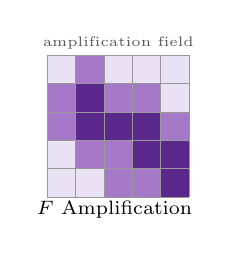
\begin{tikzpicture}[scale=0.45]
		\cellbox{purpleA}{(0,0)} \cellbox{purpleA}{(0.8,0)} \cellbox{purpleB}{(1.6,0)} \cellbox{purpleB}{(2.4,0)} \cellbox{purpleC}{(3.2,0)}
		\cellbox{purpleA}{(0,0.8)} \cellbox{purpleB}{(0.8,0.8)} \cellbox{purpleB}{(1.6,0.8)} \cellbox{purpleC}{(2.4,0.8)} \cellbox{purpleC}{(3.2,0.8)}
		\cellbox{purpleB}{(0,1.6)} \cellbox{purpleC}{(0.8,1.6)} \cellbox{purpleC}{(1.6,1.6)} \cellbox{purpleC}{(2.4,1.6)} \cellbox{purpleB}{(3.2,1.6)}
		\cellbox{purpleB}{(0,2.4)} \cellbox{purpleC}{(0.8,2.4)} \cellbox{purpleB}{(1.6,2.4)} \cellbox{purpleB}{(2.4,2.4)} \cellbox{purpleA}{(3.2,2.4)}
		\cellbox{purpleA}{(0,3.2)} \cellbox{purpleB}{(0.8,3.2)} \cellbox{purpleA}{(1.6,3.2)} \cellbox{purpleA}{(2.4,3.2)} \cellbox{purpleA}{(3.2,3.2)}
		\gridframe\rastlabel{$F$ Amplification }\smalltag{amplification field}
\end{tikzpicture}}

\newcommand{\drawClusterRaster}{%
	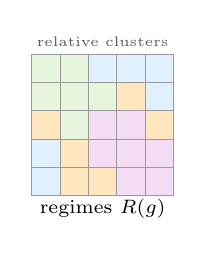
\begin{tikzpicture}[scale=0.45]
		\cellbox{clusterone}{(0,0)} \cellbox{clustertwo}{(0.8,0)} \cellbox{clustertwo}{(1.6,0)} \cellbox{clusterfour}{(2.4,0)} \cellbox{clusterfour}{(3.2,0)}
		\cellbox{clusterone}{(0,0.8)} \cellbox{clustertwo}{(0.8,0.8)} \cellbox{clusterfour}{(1.6,0.8)} \cellbox{clusterfour}{(2.4,0.8)} \cellbox{clusterfour}{(3.2,0.8)}
		\cellbox{clustertwo}{(0,1.6)} \cellbox{clusterthree}{(0.8,1.6)} \cellbox{clusterfour}{(1.6,1.6)} \cellbox{clusterfour}{(2.4,1.6)} \cellbox{clustertwo}{(3.2,1.6)}
		\cellbox{clusterthree}{(0,2.4)} \cellbox{clusterthree}{(0.8,2.4)} \cellbox{clusterthree}{(1.6,2.4)} \cellbox{clustertwo}{(2.4,2.4)} \cellbox{clusterone}{(3.2,2.4)}
		\cellbox{clusterthree}{(0,3.2)} \cellbox{clusterthree}{(0.8,3.2)} \cellbox{clusterone}{(1.6,3.2)} \cellbox{clusterone}{(2.4,3.2)} \cellbox{clusterone}{(3.2,3.2)}
		\gridframe\rastlabel{regimes $R(g)$}\smalltag{relative clusters}
\end{tikzpicture}}

\newcommand{\bigquote}[1]{%
	\begin{center}
		\begin{minipage}{0.88\linewidth}
			\centering\Large\itshape #1
		\end{minipage}
\end{center}}

\title{Adaptive margin}
\author{Stijn H. Peeters}
\date{\today}

\begin{document}
	
	\begin{frame}
		\titlepage
		\vspace{-0.8em}
	\end{frame}
	
\begin{frame}
	\begin{center}
		How do we construct a pressure manifold: a many-input device that funnels qualitatively different burdens \textit{into} an account of health?
	
		\vspace{1.2em}
		
		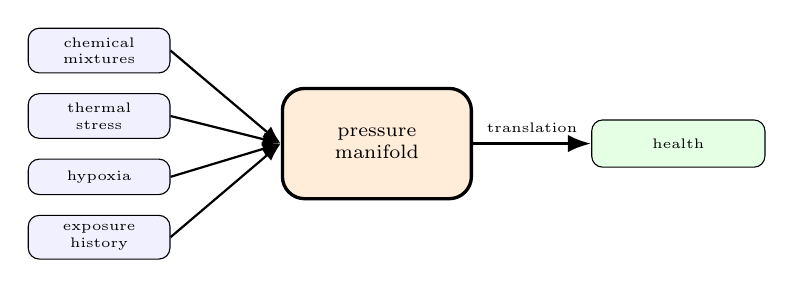
\begin{tikzpicture}[
			>=Latex,
			node distance=0.7cm,
			input/.style={
				draw,
				rounded corners,
				align=center,
				font=\tiny,
				minimum width=1.8cm,
				minimum height=0.45cm,
				fill=blue!6
			},
			manifold/.style={
				draw,
				rounded corners=8pt,
				align=center,
				font=\scriptsize,
				minimum width=2.4cm,
				minimum height=1.4cm,
				fill=orange!15,
				very thick
			},
			output/.style={
				draw,
				rounded corners,
				align=center,
				font=\tiny,
				minimum width=2.2cm,
				minimum height=0.6cm,
				fill=green!10
			}
			]
			
			% Inputs
			\node[input] (chem) {chemical\\mixtures};
			\node[input,below=0.25cm of chem] (temp) {thermal\\stress};
			\node[input,below=0.25cm of temp] (hypoxia) {hypoxia};
			\node[input,below=0.25cm of hypoxia] (memory) {exposure\\history};
			
			% Manifold
			\node[manifold,right=1.4cm of temp,yshift=-0.35cm] (man)
			{pressure\\manifold};
			
			% Output
			\node[output,right=1.5cm of man] (health)
			{health};
			
			% Arrows into manifold
			\draw[->,thick] (chem.east) -- (man.west);
			\draw[->,thick] (temp.east) -- (man.west);
			\draw[->,thick] (hypoxia.east) -- (man.west);
			\draw[->,thick] (memory.east) -- (man.west);
			
			% Arrow out
			\draw[->,very thick] (man.east) -- node[above,font=\tiny] {translation} (health.west);
			
		\end{tikzpicture}
		
		\vspace{1em}
		
		\small without resorting to \textit{regulatory} limits as the \textit{stand-in} for ``health''.
	\end{center}
\end{frame}
	
\begin{frame}
	\begin{center}
		\Large Possible solution: framing health in energetic terms.
		
		\vspace{3em}
		
		\Large But what is health? 
	\end{center}
	
	
\end{frame}

\begin{frame}{Canguilhem: health as normative capacity}
	\begin{columns}[T,onlytextwidth]
		\begin{column}{0.34\textwidth}
			
			\IfFileExists{Canguilhem.jpg}{%
				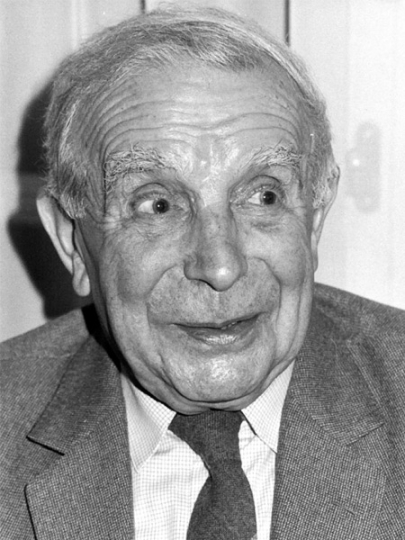
\includegraphics[width=0.82\linewidth]{Canguilhem.jpg}
			}{%
				
\begin{tikzpicture}
					\node[draw,rounded corners,minimum width=3.6cm,minimum height=4.4cm,fill=black!4,align=center] {Canguilhem\\image here};
				\end{tikzpicture}
			}
		\end{column}
		\begin{column}{0.63\textwidth}
			
			\centering
			\Large \textit{Health is normativity}
			
			\vspace{1em}

			\Large The ability of an organism to change it's \textit{state of being}
			
			\begin{block}{Main question}
				How do we go from concentrations to loss of norm-generating capacity?
			\end{block}
		\end{column}
	\end{columns}
\end{frame}

\begin{frame}{Dynamic Energy Budget Theory}
	\begin{center}
		
		\vspace{0.4em}
		
		\large  We can map stresses into DEB-like models to estimate remaining adaptive margin, the energetic latitude of the organisms to respond to the environment. 
			
		\vspace{0.8em}
		
		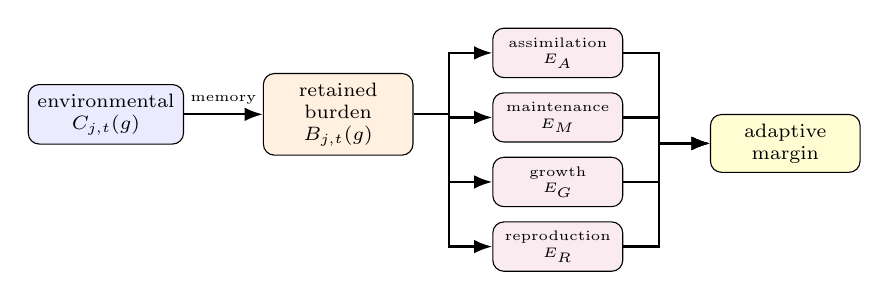
\begin{tikzpicture}[
			>=Latex,
			node distance=0.7cm,
			box/.style={
				draw,
				rounded corners,
				align=center,
				minimum width=1.9cm,
				minimum height=0.58cm,
				font=\scriptsize
			},
			axis/.style={
				draw,
				rounded corners,
				align=center,
				minimum width=1.65cm,
				minimum height=0.48cm,
				font=\tiny,
				fill=purple!8
			}
			]
			
			\node[box,fill=blue!8] (C)
			{environmental\\$C_{j,t}(g)$};
			
			\node[box,fill=orange!12,right=1.0cm of C] (B)
			{retained\\burden\\$B_{j,t}(g)$};
			
			\node[axis,right=1.0cm of B,yshift=0.78cm] (assim)
			{assimilation\\$E_A$};
			
			\node[axis,below=0.18cm of assim] (maint)
			{maintenance\\$E_M$};
			
			\node[axis,below=0.18cm of maint] (growth)
			{growth\\$E_G$};
			
			\node[axis,below=0.18cm of growth] (repr)
			{reproduction\\$E_R$};
			
			\node[box,fill=yellow!18,right=1.1cm of maint,yshift=-0.33cm] (margin)
			{adaptive\\margin};
			
			\draw[->,thick] (C) -- node[above,font=\tiny] {memory} (B);
			
			\draw[->,thick] (B.east) -- ++(0.45,0) |- (assim.west);
			\draw[->,thick] (B.east) -- ++(0.45,0) |- (maint.west);
			\draw[->,thick] (B.east) -- ++(0.45,0) |- (growth.west);
			\draw[->,thick] (B.east) -- ++(0.45,0) |- (repr.west);
			
			\draw[->,thick] (assim.east) -- ++(0.45,0) |- (margin.west);
			\draw[->,thick] (maint.east) -- ++(0.45,0) |- (margin.west);
			\draw[->,thick] (growth.east) -- ++(0.45,0) |- (margin.west);
			\draw[->,thick] (repr.east) -- ++(0.45,0) |- (margin.west);
			
		\end{tikzpicture}
		
		\vspace{0.2em}
		
		\small We thus define health as the capacity of an organism to respond to the environment. 
		
	\end{center}
\end{frame}
	

\begin{frame}{From adaptive margin to amplification}
	\begin{center}
		
		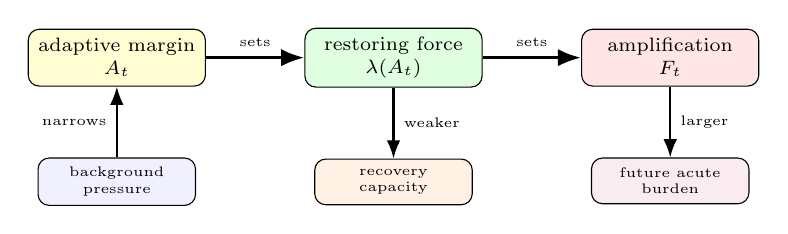
\begin{tikzpicture}[
			>=Latex,
			node distance=1.1cm,
			box/.style={
				draw,
				rounded corners,
				align=center,
				minimum width=2.25cm,
				minimum height=0.72cm,
				font=\scriptsize
			},
			smallbox/.style={
				draw,
				rounded corners,
				align=center,
				minimum width=2.0cm,
				minimum height=0.58cm,
				font=\tiny
			}
			]
			
			\node[box,fill=yellow!18] (A)
			{adaptive margin\\$A_t$};
			
			\node[box,fill=green!12,right=1.25cm of A] (lambda)
			{restoring force\\$\lambda(A_t)$};
			
			\node[box,fill=red!10,right=1.25cm of lambda] (F)
			{amplification\\$F_t$};
			
			\draw[->,very thick] (A) -- node[above,font=\tiny] {sets} (lambda);
			\draw[->,very thick] (lambda) -- node[above,font=\tiny] {sets} (F);
			
			\node[smallbox,fill=blue!6,below=0.9cm of A] (pressure)
			{background\\pressure};
			
			\node[smallbox,fill=orange!10,below=0.9cm of lambda] (recovery)
			{recovery\\capacity};
			
			\node[smallbox,fill=purple!8,below=0.9cm of F] (burden)
			{future acute\\burden};
			
			\draw[->,thick] (pressure.north) -- node[left,font=\tiny] {narrows} (A.south);
			\draw[->,thick] (lambda.south) -- node[right,font=\tiny] {weaker} (recovery.north);
			\draw[->,thick] (F.south) -- node[right,font=\tiny] {larger} (burden.north);
			
		\end{tikzpicture}
		
		\vspace{0.2em}
		
		\small
		Lower adaptive margin means weaker recovery; weaker recovery means a larger burden from the same acute event.
		
	\end{center}
\end{frame}


\begin{frame}{Environment, evidence, and adaptive margin}

	\begin{center}
		\resizebox{0.91\linewidth}{!}{%
			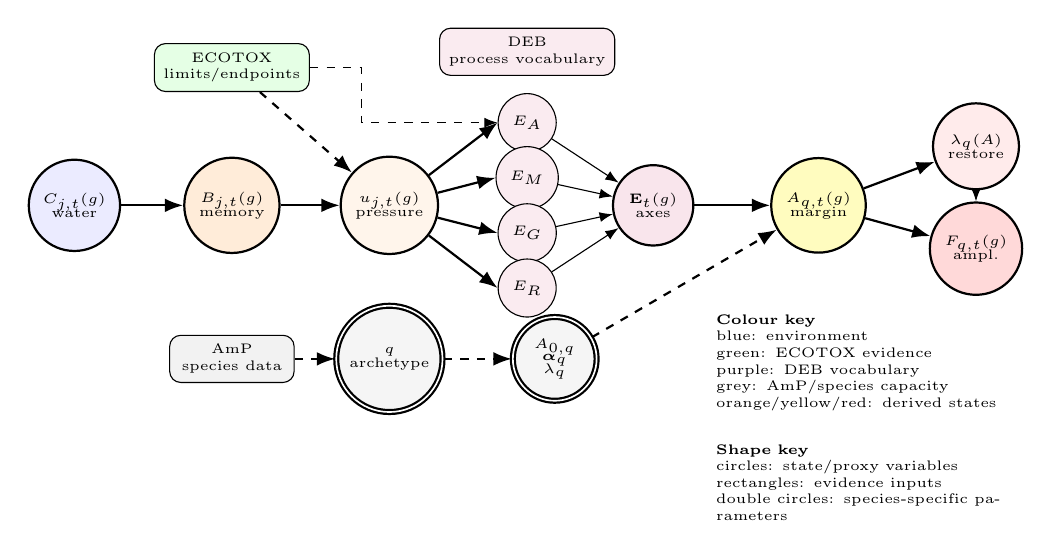
\begin{tikzpicture}[
				>=Latex,
				state/.style={
					circle,
					draw,
					thick,
					align=center,
					minimum size=1.02cm,
					font=\tiny
				},
				evidence/.style={
					rectangle,
					draw,
					rounded corners,
					align=center,
					minimum width=1.58cm,
					minimum height=0.56cm,
					font=\tiny
				},
				species/.style={
					circle,
					double,
					draw,
					thick,
					align=center,
					minimum size=1.02cm,
					font=\tiny
				},
				axisnode/.style={
					circle,
					draw,
					align=center,
					minimum size=0.72cm,
					font=\tiny
				}
				]
				
				% -------------------------------------------------------------------------
				% Main dynamic chain
				% -------------------------------------------------------------------------
				
				\node[state,fill=blue!8] (C) at (0,0)
				{$C_{j,t}(g)$\\[-0.15em]water};
				
				\node[state,fill=orange!15] (B) at (2.0,0)
				{$B_{j,t}(g)$\\[-0.15em]memory};
				
				\node[state,fill=orange!8] (U) at (4.0,0)
				{$u_{j,t}(g)$\\[-0.15em]pressure};
				
\node[axisnode,fill=purple!8] (EA) at (5.75,1.05)
{$E_A$};

\node[axisnode,fill=purple!8] (EM) at (5.75,0.35)
{$E_M$};

\node[axisnode,fill=purple!8] (EG) at (5.75,-0.35)
{$E_G$};

\node[axisnode,fill=purple!8] (ER) at (5.75,-1.05)
{$E_R$};
				
				\node[state,fill=purple!10] (Evec) at (7.35,0)
				{$\mathbf{E}_t(g)$\\[-0.15em]axes};
				
				\node[state,fill=yellow!25] (A) at (9.45,0)
				{$A_{q,t}(g)$\\[-0.15em]margin};
				
				\node[state,fill=red!15] (F) at (11.45,-0.55)
				{$F_{q,t}(g)$\\[-0.15em]ampl.};
				
				\node[state,fill=red!8] (LAMBDA) at (11.45,0.75)
				{$\lambda_q(A)$\\[-0.15em]restore};
				
				% -------------------------------------------------------------------------
				% Evidence / parameter nodes
				% -------------------------------------------------------------------------
				
				\node[evidence,fill=green!10] (ECO) at (2.0,1.75)
				{ECOTOX\\limits/endpoints};
				
				\node[evidence,fill=purple!8] (DEB) at (5.75,1.95)
				{DEB\\process vocabulary};
				
				\node[evidence,fill=black!5] (AMP) at (2.0,-1.95)
				{AmP\\species data};
				
				\node[species,fill=black!4] (Q) at (4.0,-1.95)
				{$q$\\[-0.15em]archetype};
				
				\node[species,fill=black!4] (PARAM) at (6.1,-1.95)
				{$A_{0,q}$\\[-0.2em]$\boldsymbol{\alpha}_q$\\[-0.2em]$\lambda_q$};
				
				% -------------------------------------------------------------------------
				% Main dynamic arrows: no labels
				% -------------------------------------------------------------------------
				
				\draw[->,thick] (C) -- (B);
				\draw[->,thick] (B) -- (U);
				
				\draw[->,thick] (U) -- (EA.west);
				\draw[->,thick] (U) -- (EM.west);
				\draw[->,thick] (U) -- (EG.west);
				\draw[->,thick] (U) -- (ER.west);
				
				\draw[->,thin] (EA) -- (Evec);
				\draw[->,thin] (EM) -- (Evec);
				\draw[->,thin] (EG) -- (Evec);
				\draw[->,thin] (ER) -- (Evec);
				
				\draw[->,thick] (Evec) -- (A);
				\draw[->,thick] (A) -- (LAMBDA);
				\draw[->,thick] (A) -- (F);
				\draw[->,thin,dashed] (LAMBDA) -- (F);
				
				% -------------------------------------------------------------------------
				% Evidence arrows: dashed, no labels
				% -------------------------------------------------------------------------
				
				\draw[->,thick,dashed] (ECO) -- (U);
				
				\draw[->,thin,dashed] (ECO.east) -- ++(0.65,0) |- (EA.west);
							
				\draw[->,thick,dashed] (AMP) -- (Q);
				\draw[->,thick,dashed] (Q) -- (PARAM);
				\draw[->,thick,dashed] (PARAM) -- (A);
				
				% -------------------------------------------------------------------------
				% Compact colour and shape key
				% -------------------------------------------------------------------------
				
				\node[font=\tiny,align=left,text width=3.8cm] at (10.05,-2.0)
				{\textbf{Colour key}\\
					blue: environment\\
					green: ECOTOX evidence\\
					purple: DEB vocabulary\\
					grey: AmP/species capacity\\
					orange/yellow/red: derived states};
				
				\node[font=\tiny,align=left,text width=3.8cm] at (10.05,-3.52)
				{\textbf{Shape key}\\
					circles: state/proxy variables\\
					rectangles: evidence inputs\\
					double circles: species-specific parameters};
				
		\end{tikzpicture}}
	\end{center}

\end{frame}

	\begin{frame}{}
		\centering
		\includegraphics[width=0.8\linewidth]{full_example1.png}
	\end{frame}
	
	\begin{frame}{}
		\centering
		\includegraphics[width=0.9\linewidth]{full_example3.png}
	\end{frame}
	
	\begin{frame}{}
		\centering
		\includegraphics[width=0.9\linewidth]{dynqual_mean_F_grouped_delta_map}
	\end{frame}
	
	\begin{frame}{Closing}
		\bigquote{Mapping water quality into Dynamic Energy Budget theory allows us to:}
		\vspace{0.4em}
		\begin{center}
			\begin{itemize}
				\item Combine qualitatively different stresses into a common currency, the adaptive margin. 
				\item Make use of a \textit{positive} definition of health which applicable to any species.  
				\item Mathematically useful, regardless of philosophical stance.
				\item $\ldots$ with the caveat that it's new an not yet calibrated. 
			\end{itemize}

		\end{center}
	\end{frame}
	
\end{document}